\chapter{Developed methods for logo recognition}
\label{chap:methods}

As discussed in \autoref{chap:introduction}, the system developed in this thesis follows a pipeline consisting of two stages:
\begin{enumerate}
    \item \textbf{Object Proposal}: detection of all the logos in the image
    \item \textbf{Classification}: recognition of the class of each logo
\end{enumerate}
The first stage is done by YOLO (see \autoref{sec:yolo}), while the actual logo recognition is performed by the classifier in an incremental learning setup. The system pipeline is shown in \autoref{fig:roi_and_classification}.

\begin{figure}%
	\centering

    \begin{center}
        \includegraphics[width=\columnwidth]{images/roi+classification.drawio.png}
    \end{center}

	\caption{Pipeline of the system: the class-agnostic logo detector generates Regions of interest (ROIs), then the recognition is performed by the CIL classifier.}%
	\label{fig:roi_and_classification}%
\end{figure}

The detector used in the first stage is a class-agnostic logo detector: it is a logo detector since it only detects logos in the image; and it is class-agnostic since the number of classes detected is only one. In fact, in this first stage the detector will be responsible for finding any generic logo (i.e., a single class) in the image. This is a crucial aspect if we seek to achieve incremental learning logo recognition, because in this way detection can be decoupled from recognition. If the logo detector localizes any generic logo in the image, and delegates the actual recognition to the CIL classifier, there is no need to develop an incremental learning detector as well.

An important aspect of the classifier is the size of the model (in terms of the number of parameters). To this reason, a part of this work aims to decrease the number of parameters of the classifier using two different techniques. The first one is described in \autoref{sec:method-pruning}, using masking and pruning introduced in \autoref{sec:masking-pruning} it aims to prune the model after the training of each incremental step, thus reducing the number of parameters. The second technique is the Knowledge Distillation (KD) described in \autoref{sec:method-kd}, where a smaller model is trained with the supervision of a bigger model trained on the same task.

The code developed in this thesis is available in the GitHub repository\footnote{GitHub repository with the code developed in this thesis: \\ \href{https://github.com/gianlucagiudice/logo-detection-recognition}{https://github.com/gianlucagiudice/logo-detection-recognition}} linked below. The system is developed using the Python programming language, and the code is implemented using PyTorch \cite{paszke2019pytorch}, a widely used deep learning framework. The training of the models is done using the NVIDIA Tesla K80 GPU with 12GB of memory.

\vspace{1.5\baselineskip}
This chapter describes all the details about the logo detector in \autoref{sec:method-roi} and continues with the classifier in \autoref{sec:method-classifier}. Then, in \autoref{sec:method-pruning} and \autoref{sec:method-kd} are discussed some techniques to reduce the number of model parameters. In order to evaluate the drop in performance of the CIL classifier when compared to a standard close-set classification task (i.e. all classes are available from the beginning and no new ones are introduced over time),
the chapter ends in \autoref{sec:method-baseline} with the introduction of different baselines.

\section{Region proposal}
A key component of the system is the logo detector. Formally, this first step is an object detection task, where the objects to be detected are the logos in the image. The logo detector outputs the coordinates of the bounding boxes corresponding to the logos in the image.
Bounding boxes can be used to crop the portions of the image creating regions of interest (ROIs).
ROIs correspond to what the detector considers a generic logo and can be used directly as input to the CIL model that classifies (i.e. recognizes) the logo.

\label{sec:method-roi}
\subsection{YOLOv5m6}
The class-agnostic logo detector is based on YOLOv5-v6.0 \cite{glenn_jocher_2021_5563715}.
There are different versions of YOLOv5-v6.0, depending on the size of the model and the size of the input image.
In general, larger models perform better, with the disadvantage of longer training time, longer inference time and more computational resources required to train the model.
On the other hand, a small model might achieve very low performance, thus misleading the final evaluation of the system that relies heavily on the detector.
Therefore, a model that is too small could act as a bottleneck for the whole system. A more detailed analysis of this trade-off is shown in \autoref{fig:yolo-sizes} and \autoref{table:yolo-sizes}.

\begin{figure}
	\centering

    \begin{center}
        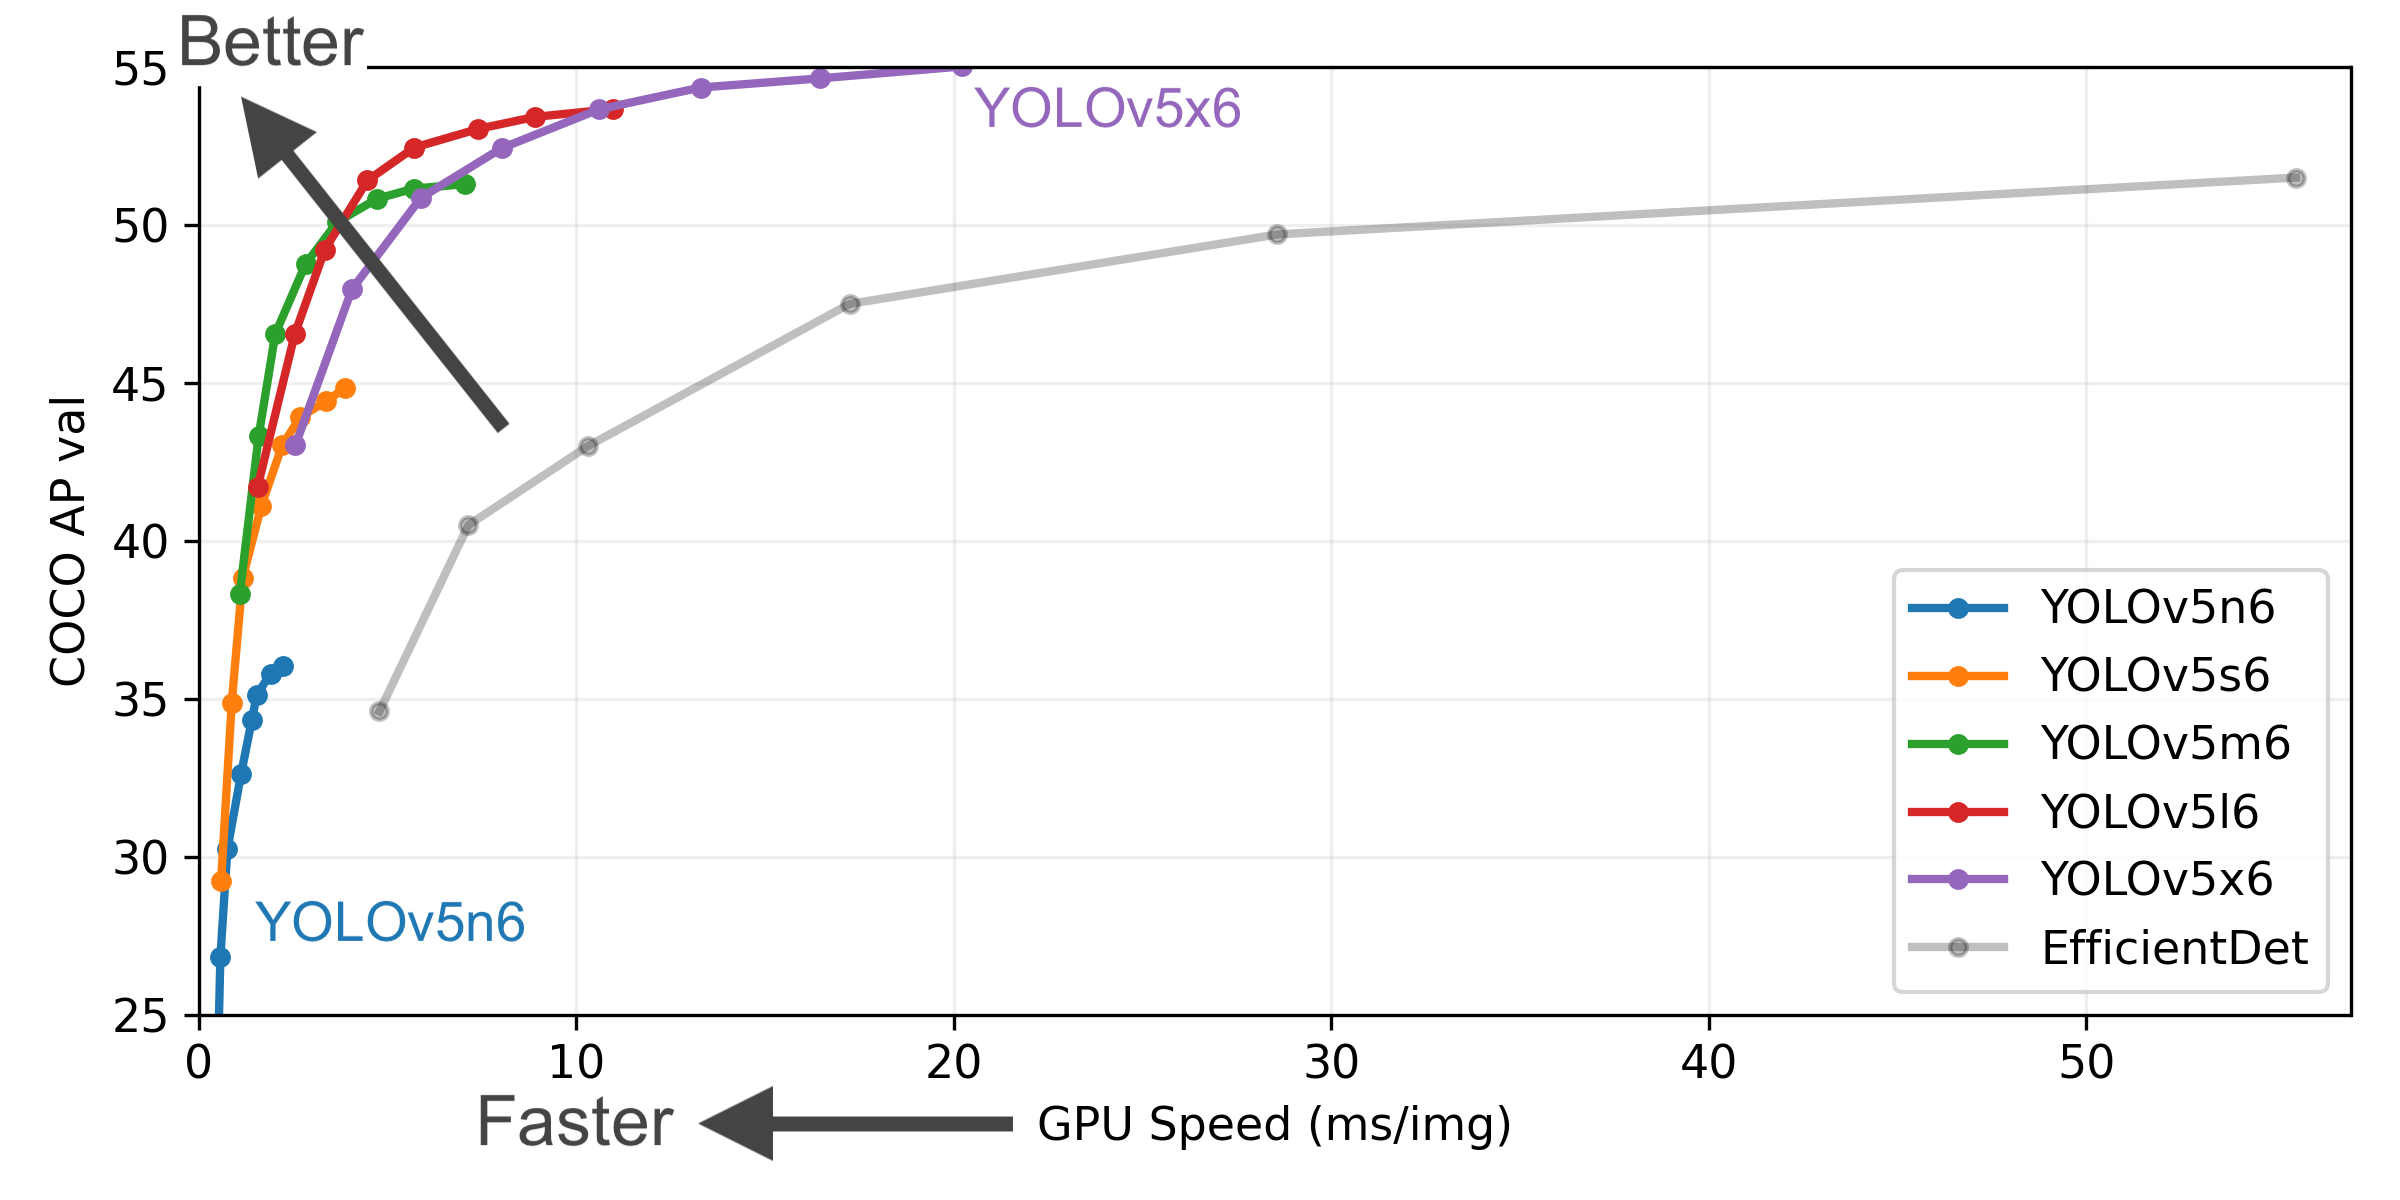
\includegraphics[width=0.9\columnwidth]{images/yolov5-sizes.png}
    \end{center}

	\caption{Performance and speed comparison for the YOLOv5-v6.0 family of models considering the mAP@0.5:0.95 metric measured on the 5000-image COCO val2017 \cite{lin2014microsoft} dataset. The plot shows the performance of different models varying the input size of the image from $256 \times 256$px to $1536 \times 1536$px. Image from \cite{glenn_jocher_2021_5563715}.}
	\label{fig:yolo-sizes}%
\end{figure}


\begin{table}
    \centering
    \centerline{\begin{tabular}{c|c|c|c|c|c|c|c}
        \hline
        \multirow{2}{*}{ \textbf{Model}} & 
        \textbf{size} &
        \textbf{$\text{mAP}^{\text{val}}$} & 
        \textbf{$\text{mAP}^{\text{val}}$} & 
        \textbf{Speed} & 
        \textbf{Speed} & 
        \textbf{\# params} & 
        \textbf{FLOPs} \\
        & (pixels) & \textbf{0.5:0.95} & \textbf{0.5} & \textbf{CPU} (ms) & \textbf{GPU} (ms) & (M) & @640px (B) \\
        \hline
        YOLOv5n & 640 & 28.0 & 45.7 & 45 & 6.3 & 1.9 & 4.5 \\
        YOLOv5s & 640 & 37.4 & 56.8 & 98 & 6.4 & 7.2 & 16.5 \\
        YOLOv5m & 640 & 45.4 & 64.1 & 224 & 8.2 &  21.2 & 49.0 \\
        YOLOv5l & 640 & 49.0 & 67.3 & 430 & 10.1 & 46.5 & 109.1 \\
        YOLOv5x & 640 & 50.7 & 68.9 & 766 & 12.1 & 86.7 & 205.7 \\
        \hline
        YOLOv5n6 & 1280 & 36.0 & 54.4 & 153 & 8.1 & 3.2 & 4.6 \\
        YOLOv5s6 & 1280 & 44.8 & 63.7 & 385 & 8.2 & 12.6 & 16.8 \\
        YOLOv5m6 & 1280 & 51.3 & 69.3 & 887 & 11.1 &  35.7 & 50.0 \\
        YOLOv5l6 & 1280 & 53.7 & 71.3 & 1784 & 15.8 & 76.8 & 111.4 \\
        YOLOv5x6 & 1280 & 55.0 & 72.7 & 3136 & 26.2 & 140.7 & 209.8 \\
        \hline        
        \end{tabular}}
    \caption{Performance comparison considering the mAP@0.5:0.95 metric of all checkpoints of YOLOv5-v6.0 trained for 300 epochs on COCO dataset \cite{glenn_jocher_2021_5563715}.}
    \label{table:yolo-sizes}
\end{table}

The class-agnostic logo detector is based on YOLOv5m6, shown in \autoref{table:yolo-sizes}, with an image input size of $512 \times 512$px and pre-trained on the COCO dataset.
The model is then finetuned for 30 epochs on the task of class-agnostic logo detection.

\section{Classification}
\label{sec:method-classifier}
Given the ROIs, the classification of each cropped region is performed by a model trained using CIL techniques. To achieve this goal, the classifier is trained using the DER algorithm \cite{yan2021dynamically} described in \autoref{sec:der-algorithm}.

\subsection{ResNet-34}
\label{sec:resnet}
The DER algorithm introduces a new feature extractor $\mathcal{F}_t$ at each incremental step. This feature extractor consists of a CNN. In the developed system, the backbone of the CNN, used as feature extractor, is ResNet-34 \cite{he2016deep} pre-trained on ImageNet1000 \cite{deng2009imagenet}.

The peculiar aspects of ResNet architecture are the Residual Connections, shown in \autoref{fig:residual-connection}.
These connections are types of skip-connection that, instead of learning unreferenced functions, learn residual functions with respect to the layer inputs.
Formally, denoting the desired underlying mapping as $\mathcal{H}(x)$, we let the stacked nonlinear layers fit another mapping of $\mathcal{F}(x) := \mathcal{H}(x) - x$. The original mapping is recast into $\mathcal{F}(x) + x$.

The intuition is that it is easier to optimize the residual mapping instead of optimizing the original, unreferenced mapping. In the extreme case, if an identity mapping is optimal, it is easier to push the residual to zero than to fit an identity mapping using a stack of non-linear layers \cite{he2016deep}.

The architecture of ResNet-34, shown in \autoref{table:resnet}, consists of multiple stacked building blocks. Each building block, represented by the brackets in \autoref{table:resnet}, adopts the residual connection described above.
The combination of both skip-connection and batch-normalization (BN) \cite{ioffe2015batch} in ResNet enable the training of a very deep neural network, achieving high performance.
The total number of parameters of ResNet-34 used as feature extractor at each incremental step is 23 million.

\begin{table}
    \centering
    \begingroup
    
    \begin{tabular}{>{\centering\arraybackslash}p{.3\textwidth}|>{\centering\arraybackslash}p{.3\textwidth}|>{\centering\arraybackslash}p{.3\textwidth}}


        \hline
        \multicolumn{3}{c}{\textbf{ResNet-34 architecture}}\\
        \hline
        \textbf{Layer name} & \textbf{Output size} & \textbf{Layer} \\
        \hline
        \hline
        conv1 & $112 \times 122$ & $7 \times 7, 64,$ stride $2$ \\
        \hline
          & $56 \times 56$ & $3 \times 3$ max pool, stride $2$ \\
        \hline

        \[ \textrm{conv2\char`_x} \] &  \[56 \times 56 \] & \[\left[ \begin{array}{c} 3 \times 3, \, 64\\ 3 \times 3, \, 64  \end{array}\right] \times 3 \]\\
        \hline

        \[ \textrm{conv3\char`_x} \] &  \[28 \times 28 \] & \[\left[ \begin{array}{c} 3 \times 3, \, 128\\ 3 \times 3, \, 128  \end{array}\right] \times 4 \]\\
        \hline

        \[ \textrm{conv4\char`_x} \] &  \[14 \times 14 \] & \[\left[ \begin{array}{c} 3 \times 3, \, 256\\ 3 \times 3, \, 256  \end{array}\right] \times 6 \]\\
        \hline

        \[ \textrm{conv5\char`_x} \] &  \[7 \times 7 \] & \[\left[ \begin{array}{c} 3 \times 3, \, 512\\ 3 \times 3, \, 512  \end{array}\right] \times 3 \]\\
        \hline
        & $1000 \times 1$ & average pool \\
        \hline
        FC & $1000 \times 1$ & $1000$-d FC layer, softmax \\
        \hline
        \end{tabular}
    \endgroup
    \caption{Architecture of ResNet-34, the brackets represent a stack of building blocks. }
    \label{table:resnet}
\end{table}

\begin{figure}%
	\centering
	\subfloat[\centering Residual learning: a building block]{{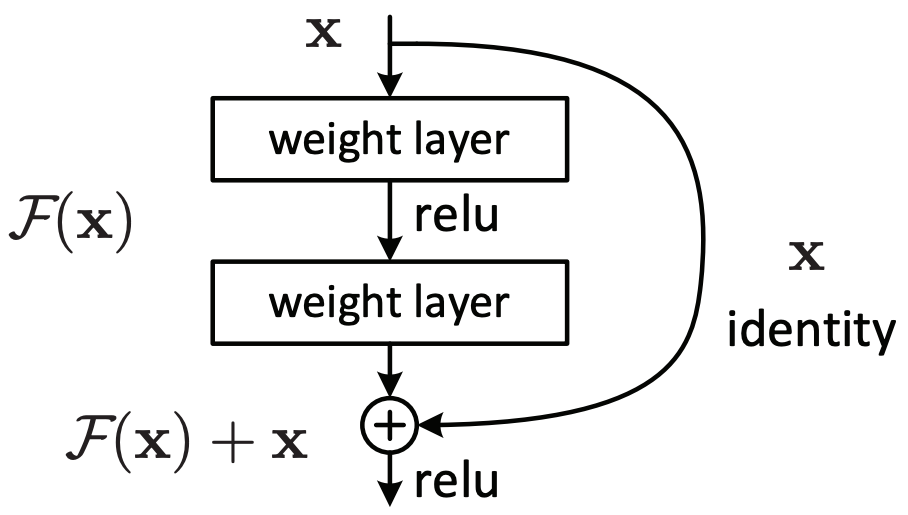
\includegraphics[width=0.45\textwidth]{images/residual-theory.png} }}%
	\hfill
	\subfloat[ An example of residual connection in a building block. This building block corresponds to \textrm{conv2\char`_x} in \autoref{table:resnet} ]{{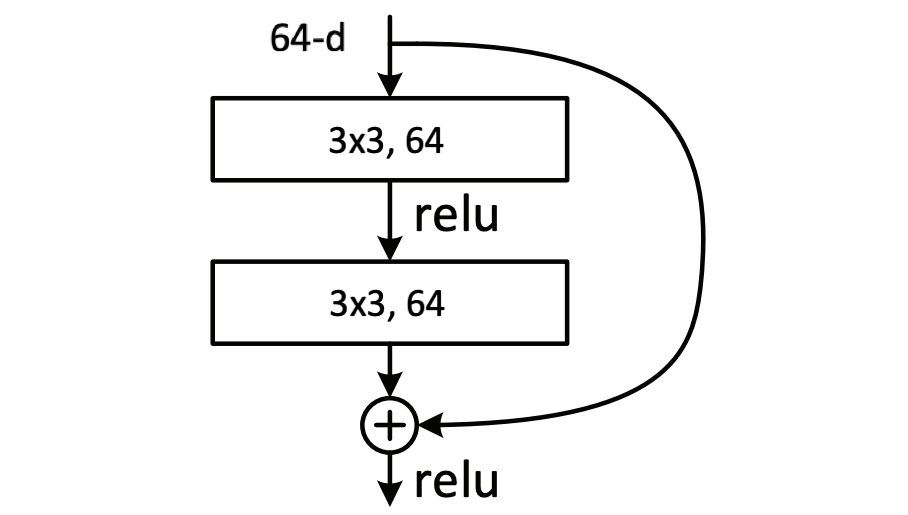
\includegraphics[width=0.45\textwidth]{images/residual-practice.png} }}%
	\caption{Residual connection in ResNet architecture \cite{he2016deep}.}%
	\label{fig:residual-connection}%
\end{figure}

\subsection{CIL classifier}
%The classifier is developed in a CIL setup. This makes it possible to recognise new logos by enriching old knowledge. The algorithm used for CIL is the DER algorithm described in \autoref{sec:der-algorithm}.
An implementation of the DER algorithm is provided by PyCIL\footnote{PyCIL GitHub repository: \\ \href{https://github.com/G-U-N/PyCIL}{https://github.com/G-U-N/PyCIL}} (see \autoref{sec:pycil}), and is used as a starting point for the development of the CIL classifier. 
All the changes made to the implementation of DER in PyCIL are described in the following sections, and can be found in this\footnote{GitHub repository relative to the CIL model of this thesis: \\ \href{https://github.com/gianlucagiudice/PyCIL}{https://github.com/gianlucagiudice/PyCIL}} GitHub repository.

The implementation of DER in PyCIL reflects the description given in the DER paper, with only one difference to the third phase of the DER algorithm (called 'classifier learning phase' in \autoref{sec:der-algorithm}). 
In fact, in PyCIL the 'Classifier Learning Stage' is performed using the WA described in \autoref{sec:wa-biased}; in this way it is possible to solve the problem of biased weights in the FC layer without the need to train the model further.
It is important to emphasize that, although this step of the algorithm is modified, the final performance reported by PyCIL is very similar to that obtained from the original DER paper (see \autoref{table:cil-results}).

\subsection{Regularization techniques}
To avoid model overfitting, the architecture of the NN created with the DER algorithm is modified.
Starting from the original architecture, a dropout layer is added before the FC layer represented in \autoref{fig:der-pipeline} by the classifier $\mathcal{H}_t$.

\subsubsection{Dropout}
\label{sec:methods-dropout}
DNNs with a large number of parameters are prone to overfitting the training data and do not generalize well on the test set.
Dropout \cite{srivastava2014dropout} is a technique to address this problem.

At training time, the units of the NN, along with their connections, are dropped randomly with a given probability $p$ (a common value is $p = 0.5$). At test time, all units are present, but with weights scaled by $p$ (i.e. $w$ becomes $pw$). This procedure is shown in \autoref{fig:dropout}.

The idea is to prevent co-adaptation, where the NN becomes too reliant on particular connections, as this could be a symptom of overfitting. Intuitively, the dropout can be considered as the creation of an implicit ensemble of NNs.

\begin{figure}%
	\centering
	\subfloat[\centering Standard neural network]{{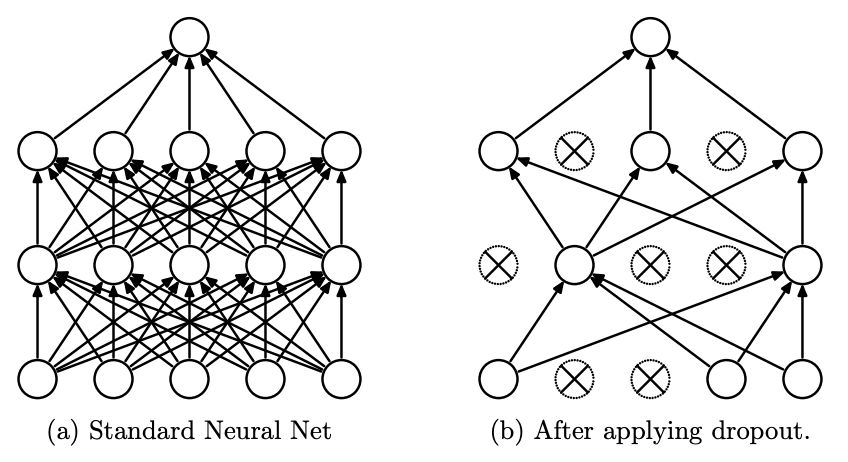
\includegraphics[width=0.30\textwidth,trim={0 24 220 0},clip]{images/dropout.png} }}%
	\hspace*{2cm}
	\subfloat[\centering Neural network after applying dropout ]{{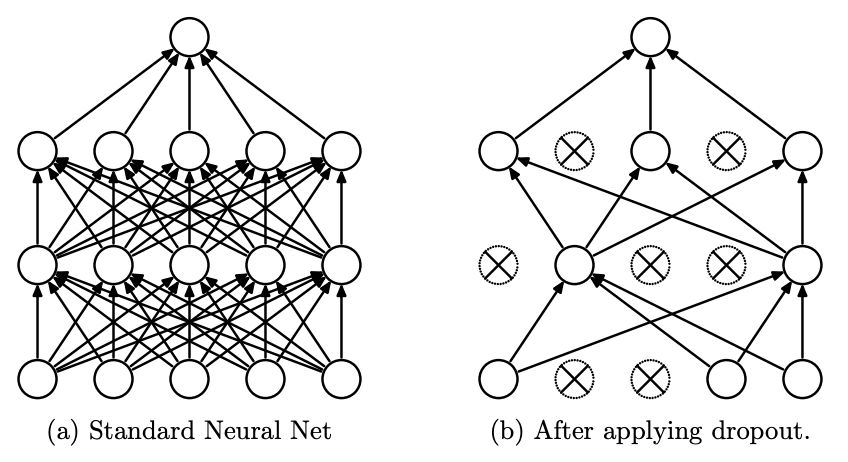
\includegraphics[width=0.30\textwidth,trim={220 24 0 0},clip]{images/dropout.png} }}%
	\caption{Dropout mechanism in a Neural Network with 2 hidden layers \cite{srivastava2014dropout}.}%
	\label{fig:dropout}%
\end{figure}

\subsection{Data augmentation}
\label{sec:methods-augment}
As discussed in \autoref{sec:dataset-stat}, one problem with the LogoDet-3K dataset is that some classes have a low number of images. Moreover, as shown in \autoref{table:logodet3k-quartile}, these classes are not an exception but the majority of those in the dataset. In fact, 50\% of the dataset has a number of images less than or equal to 54.

Training a model using a small number of examples per class can be a problem in machine learning in general, but this is particularly true in the deep learning domain, where models require a huge amount of data.

Image augmentation is a data augmentation method that generates more training data from the existing training samples.
This is a very useful technique to address the problem of low number of images per class in LogoDet-3K.
In addition, data augmentation is another way to avoid overfitting, as it creates synthetic samples by adding random perturbations to the original image yet preserving its main characteristics, thus achieving better generalization.

The type of data augmentation adopted during the training of the model is called online data augmentation.
This technique consists of applying a random transformation to the original image before feeding it to the model.
In this way, it is theoretically possible to obtain an infinitely large dataset. The process of data augmentation is heavily dependent on the type of transformations applied to the images: an excessive transformation of the original image may mislead the model in learning the main features of the image, while keeping the image as similar as possible to the original one may have the same effect as not applying data augmentation at all.

The transformations used to augment the original dataset, shown in \autoref{fig:example-augmentation}, and used to train the CIL classifier are the following:
\begin{itemize}
    \item \textbf{Geometric transformations}:
    \begin{itemize}
        \item \textbf{Random affine}: transforms the image while keeping the centre invariant.
        \item \textbf{Random perspective}: perspective transformation of the image.
    \end{itemize}
    \item \textbf{Color transformations}:
    \begin{itemize}
        \item \textbf{Adjust sharpness}: transforms the original image into a sharper one according to the sharpening factor. This parameter is chosen a priori and is fixed for each transformation.
        \item \textbf{Posterize}: reduces the number of bits for each color channel.
        \item \textbf{Color jitter}: randomly changes the brightness, contrast, saturation and hue of an image.
    \end{itemize}
\end{itemize}

As previously stated, the data augmentation is performed in an online manner, in this way it is possible to obtain a slightly different image at each training epoch of the model.
The original image is transformed using the transformations listed above, but the final image is a combination of geometric and color transformations. 
This procedure is shown in \autoref{fig:data_augmentation}, and is applied to different logos in \autoref{fig:final_data_augmentation}.

\begin{figure}[H]
	\centering

    \begin{center}
        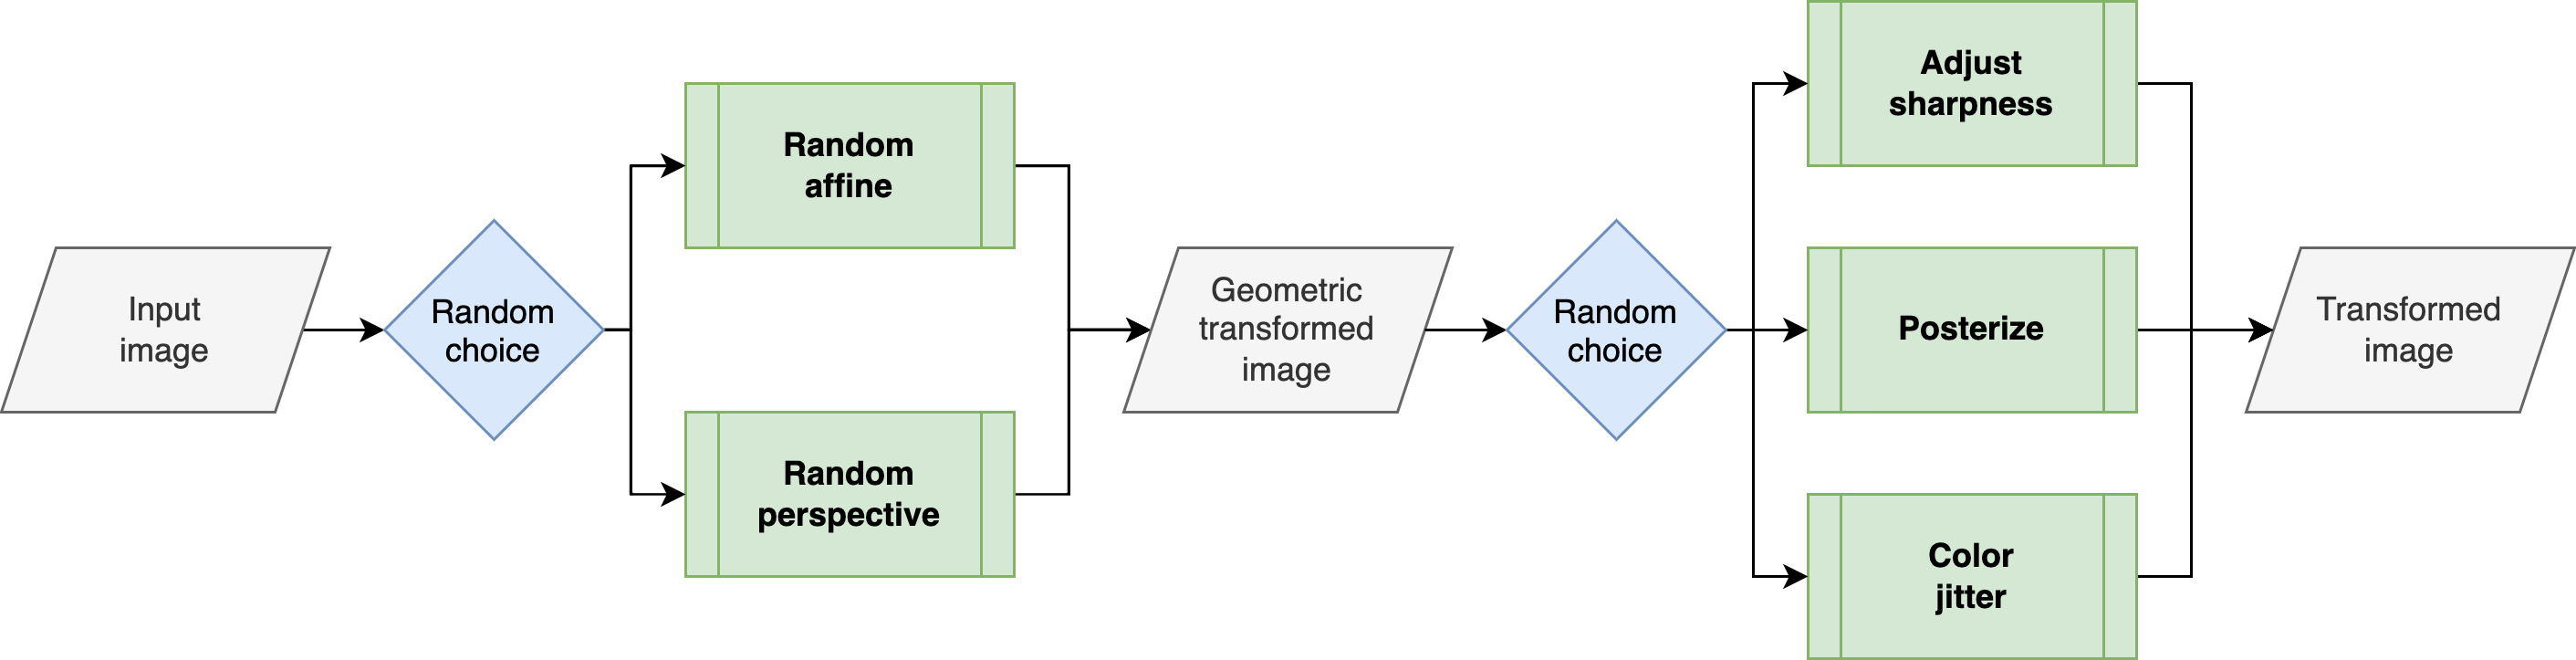
\includegraphics[width=\columnwidth]{images/data_augmentation.drawio.png}
    \end{center}

	\caption{Image transformation pipeline for data augmentation: first the input image is transformed via a geometric transformation, then a color transformation is applied.}%
	\label{fig:data_augmentation}%
\end{figure}

\newpage

\begin{figure}[H]
    \centering
    \subfloat[Original image]{{
\includegraphics[height=3cm]{images/augmentations/original.jpg} }}%
    \hfill
    \subfloat[Random affine transformation]{{
\includegraphics[height=3cm]{images/augmentations/affine.jpg} }}%
    \hfill
    \subfloat[Random perspective transformation]{{
\includegraphics[height=3cm]{images/augmentations/perspective.jpg} }}%
    \hfill
    \subfloat[Adjust sharpness]{{
\includegraphics[height=3cm]{images/augmentations/sharpness.jpg} }}%
    \hspace*   {2cm}
    \subfloat[Posterize]{{
\includegraphics[height=3cm]{images/augmentations/posterize.jpg} }}%
    \hfill
    \subfloat[Random color Jitter]{{
\includegraphics[height=3cm]{images/augmentations/color_jitter.jpg} }}%
    \caption{Examples of image transformations. The transformations (d) and (e) are shown in a single image since, given the sharpness factor and the number of bin for the posterization, the result of the transformation is always the same.}%
    \label{fig:example-augmentation}%
\end{figure}

\begin{figure}[H]
	\centering
	\subfloat[Logo 1]{{
\includegraphics[height=2cm]{images/augmentations/transf1.png} }}%
	\hfill
	\subfloat[Logo 2]{{
\includegraphics[height=2cm]{images/augmentations/transf2.png} }}%
	\hfill
	\subfloat[Logo 3]{{
\includegraphics[height=2cm]{images/augmentations/transf3.png} }}%
	\hfill
	\subfloat[Logo 4]{{
\includegraphics[height=2cm]{images/augmentations/transf4.png} }}%
	\hfill
    \subfloat[Logo 5]{{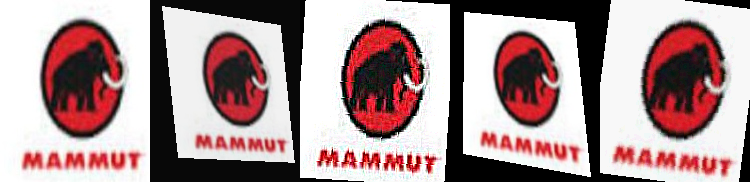
\includegraphics[height=2cm]{images/augmentations/transf5.png} }}%
	\hfill
    \subfloat[Logo 6]{{
\includegraphics[height=2cm]{images/augmentations/transf6.png} }}%
	\caption{Examples of data augmentation on different logos: the first column represents the original image, the other columns are some transformation applied to the original image following the pipeline described in \autoref{fig:data_augmentation}.}%
	\label{fig:final_data_augmentation}%
\end{figure}

\subsection{Training}
The training of the CIL model can be divided into two main steps: the initial task and the iterations of CIL. In the initial task the model is trained for 200 epochs, while for the incremental learning iterations it is trained for 150 epochs.

The number of training epochs in the initial task is higher because in this phase the network requires a longer time to converge, this is due to these two factors: the neural network must adapt the weights trained on ImageNet to the logo classification task;
it is assumed that the number of classes at the initial task is greater than the number of classes introduced at each incremental learning iteration.

\subsubsection{Early stopping}
Early stopping is used to avoid overfitting of the model.
This is done by monitoring the accuracy of the model during training on the validation set.
The hyperparameters of early stopping are the following: the number of epochs with no improvement after which training will be stopped is set to 30 (i.e. patience); the minimum change in the monitored accuracy to be considered as an improvement is set to 0.5\% (i.e., the minimum delta).

\subsubsection{SGD optimizer}
\label{sec:sgd_opt}
To update the model weights two different optimizers are tested.
One of them is Stochastic Gradient Descent (SGD), an iterative method for optimizing an objective function.

As described in \cite{zhang2021dive}, in deep learning the objective function is usually the average of the loss functions for each example in the training dataset. Given a training dataset of $n$ examples, we assume that $f_i(\textbf{w})$ is the loss function with respect to the training example of index $i$, where $\textbf{w}$ is the parameter vector. Then the objective function is given by:
\begin{equation}
    f(\textbf{w}) = \frac{1}{n} \sum_{i=1}^n f_i(\textbf{w})
\end{equation}
The gradient of the objective function at $\textbf{w}$ is computed as:
\begin{equation}
    \nabla f(\textbf{w}) = \frac{1}{n} \sum_{i=1}^n \nabla f_i(\textbf{w})
\end{equation}
If gradient descent is used, the computational cost for each independent iteration is $\mathcal{O}(n)$, which grows linearly with $n$. Therefore, when the training dataset is larger, the cost of gradient descent for each iteration will be higher.

SGD reduces the computational cost at each iteration by uniformly sampling an index $i \in \{ 1, \, ..., \, n\}$ from data examples, and computes the gradient $\nabla f_i (\textbf{w})$ to update $\textbf{w}$:

\begin{equation}
    \textbf{w} \leftarrow \textbf{w} - \eta \nabla f_i(\textbf{w})
\end{equation}
where $\eta$ is the learning rate ($\eta = 0.1$ in the experiments described in \autoref{chap:experiments}). In this way the computational cost for each iteration drops from $\mathcal{O}(n)$ of the gradient descent to the constant $\mathcal{O}(1)$ of SGD. Moreover, the stochastic gradient $\nabla f_i(\textbf{w})$ is an unbiased estimate of the full gradient $\nabla f(\textbf{w})$ because:
\begin{equation}
    \mathbb{E}_i \nabla f_i(\mathbf{w}) = \frac{1}{n} \sum_{i = 1}^n \nabla f_i(\mathbf{w}) = \nabla f(\mathbf{w})
\end{equation}
This means that, on average, the stochastic gradient is a good estimate of the gradient.

A compromise between computing the true gradient and the gradient with a single sample is to compute the gradient against more than one training sample (called a 'mini-batch'). This means replacing the gradient $\nabla f_i(\textbf{w})$ on a single observation with one over a small batch $\mathcal{B}_t = \{ \textbf{x}^{(1)},\, ..., \, \textbf{x}^{(m)}\}$ (for the experiments described in \autoref{chap:experiments}, $|\mathcal{B}_t| = 2048$). Then, the gradient $\textbf{g}_t$ over a small batch $\mathcal{B}_t$ is given by:
\begin{equation}
    \mathbf{g}_t = \frac{1}{|\mathcal{B}_t|} \sum_{i \in \mathcal{B}_t} \nabla f_i(\mathbf{w})
\end{equation}
Note that, in an epoch, the examples are not reused for multiple batches. The minibatch SGD algorithm is shown in \autoref{alg:sgd} as described by Goodfellow et al. in \cite{Goodfellow-et-al-2016}.


\begin{algorithm}
    \caption{SGD algorithm with minibatches}\label{alg:sgd}
    \begin{algorithmic}
        \Require Learning rate $\eta$
        \Require Initial parameters $\textbf{w}$
        
    \While{stopping criterion not met}
        
        Sample a minibatch $\mathcal{B}$ of $m$ examples from the training set $\{ \textbf{x}^{(1)},\, ..., \, \textbf{x}^{(m)}\}$ with corresponding labels $\textbf{y}^{(i)}$.

    Compute gradient estimate: $\hat{\mathbf{g}} = \frac{1}{|\mathcal{B}|} \sum_{i \in \mathcal{B}_t} \nabla f_i(\mathbf{w})$.

    Apply update: $\textbf{w} \leftarrow \textbf{w} - \eta \hat{\mathbf{g}}$.

    \EndWhile
    \end{algorithmic}
    \end{algorithm}


\subsubsection{Adam optimizer}
\label{sec:adam_opt}
The second optimizer used in the experiments is Adam \cite{kingma2014adam}, which can be considered as a combination of RMSProp \cite{hinton2012neural} and momentum \cite{sutskever2013importance}. Adam is an adaptive learning rate optimizer, i.e. it uses a separate learning rate for each parameter and automatically adapts these learning rates throughout the course of learning. A key component of Adam is that it uses exponential weighted moving averages (also known as leaky averaging) to obtain an estimate of the momentum and the second moment of the gradient.

To estimate the first-order and the second-order moments of the gradient, Adam uses two state variables:
\begin{equation}
    \begin{split}\begin{aligned}
        \mathbf{v}_t & \leftarrow \beta_1 \mathbf{v}_{t-1} + (1 - \beta_1) \mathbf{g}_t \\
        \mathbf{s}_t & \leftarrow \beta_2 \mathbf{s}_{t-1} + (1 - \beta_2) \mathbf{g}_t^2
    \end{aligned}\end{split}
\end{equation}
where $\beta_1$ and $\beta_2$ are nonnegative weighting parameters. In the experiments in \autoref{chap:experiments}, $\beta_1=0.9$ and $\beta_2=0.999$.

Initially, both $\mathbf{v}_0$ and $\mathbf{s}_0$ are set to 0, resulting in a bias towards smaller values. For this reason, Adam computes the bias-corrected $\hat{\mathbf{v}}_t$ and $\hat{\mathbf{s}}_t$ as follows:
\begin{equation}
    \begin{split}\begin{aligned}
        \hat{\mathbf{v}}_t & = \frac{\mathbf{v}_t}{1 - \beta_1^t} \\
        \hat{\mathbf{s}}_t & = \frac{\mathbf{s}_t}{1 - \beta_2^t}
    \end{aligned}\end{split}
\end{equation}
Then, the gradient is rescaled accordingly to consider both the first-order and second-order moments:
\begin{equation}
    \mathbf{g}_t' = \eta \frac{ \hat{\mathbf{v}}_t}{\sqrt{\hat{\mathbf{s}}_t} + \epsilon}
\end{equation}
where, $\eta$ is the learning rate (set to $0.001$ in the experiments in \autoref{chap:experiments}) and $\epsilon = 10^{-8}$ is a constant to achieve numerical stability.

Finally, the parameters are updated as follows:
\begin{equation}
    \textbf{w}_t \leftarrow \textbf{w}_{t-1} - \mathbf{g}_t'
\end{equation}

The Adam algorithm is shown in \autoref{alg:adam} as described by Goodfellow et al. in \cite{Goodfellow-et-al-2016}.

\begin{algorithm}
    \caption{The Adam algorithm}\label{alg:adam}
    \begin{algorithmic}
        \Require Learning rate $\eta$
        \Require Exponential decay rates for moment estimates, $\beta_1$ and $\beta_2$ in $[0, \, 1)$ (Suggested defaults: $0.9$ and $0.999$ respectively).
        \Require Small constant $\epsilon$ used for numerical stabilization (Suggested default: $10^{-8}$).
        \Require Initial parameters $\textbf{w}$\\
        Initialize 1st and 2nd moment variable $\mathbf{s} = 0$, $\mathbf{r} = 0$\\
        Initialize time step $t = 0$
    \While{stopping criterion not met}
        
        Sample a minibatch $\mathcal{B}$ of $m$ examples from the training set $\{ \textbf{x}^{(1)},\, ..., \, \textbf{x}^{(m)}\}$ with corresponding labels $\textbf{y}^{(i)}$.
        
        Compute gradient estimate: $\hat{\mathbf{g}} = \frac{1}{|\mathcal{B}|} \sum_{i \in \mathcal{B}_t} \nabla f_i(\mathbf{w})$.

        $t \leftarrow t +1$
        
        Update biased first moment estimate: $\mathbf{v} \leftarrow \beta_1 \mathbf{v} + (1 - \beta_1) \mathbf{\hat{g}}$

        Update biased second moment estimate: $\mathbf{s} \leftarrow \beta_2 \mathbf{s} + (1 - \beta_2) \mathbf{\hat{g}}^2$

        Correct bias in first moment: $\hat{\mathbf{v}} = \frac{\mathbf{v}}{1 - \beta_1^t}$
  
        Correct bias in second moment: $\hat{\mathbf{s}} = \frac{\mathbf{s}}{1 - \beta_2^t}$

        Compute update: $\Delta \mathbf{w} = \eta \frac{ \hat{\mathbf{v}}}{\sqrt{\hat{\mathbf{s}}} + \epsilon}$

        Apply update: $\textbf{w} \leftarrow \textbf{w} - \Delta \mathbf{w}$.

    \EndWhile
    \end{algorithmic}
    \end{algorithm}

\subsubsection{Learning rate decay}
For both SGD and Adam, an exponential decay scheduling is applied to the learning rate: once one epoch reaches one of the predetermined epochs (called milestones) the learning rate of the optimizer is multiplied by a factor $\gamma = 0.1$. For the training of the CIL classifier, the milestones are set to 60, 100 and 150 for the initial task, and to 40, 75 and 100 for each incremental learning iteration.

Adjusting the learning rate is an important aspect of the optimization process. Some of the motivations behind learning rate scheduling are described below:
\begin{itemize}
    \item The magnitude of the learning rate is a key factor in the optimization procedure: if the learning rate is too large, optimization diverges, while if it is too small, either training takes too long or a suboptimal result is achieved.
    \item If the learning rate remains high, the algorithm may bounce around the minimum or even jump over it and thus failing to reach optimality. 
\end{itemize}

The learning rate decay is used to train models for the experiments described in \autoref{chap:experiments}. An example of the effect of the learning rate decay is shown in \autoref{fig:lr_decay}.
By plotting the accuracy of the model at each training epoch, it is possible to notice that, when a milestone is reached (epoch 60) and the learning rate is scaled by a factor of $10^{-1}$, there is an improvement in the accuracy of the model in subsequent epochs.

\begin{figure}[H]
	\centering

    \begin{center}
        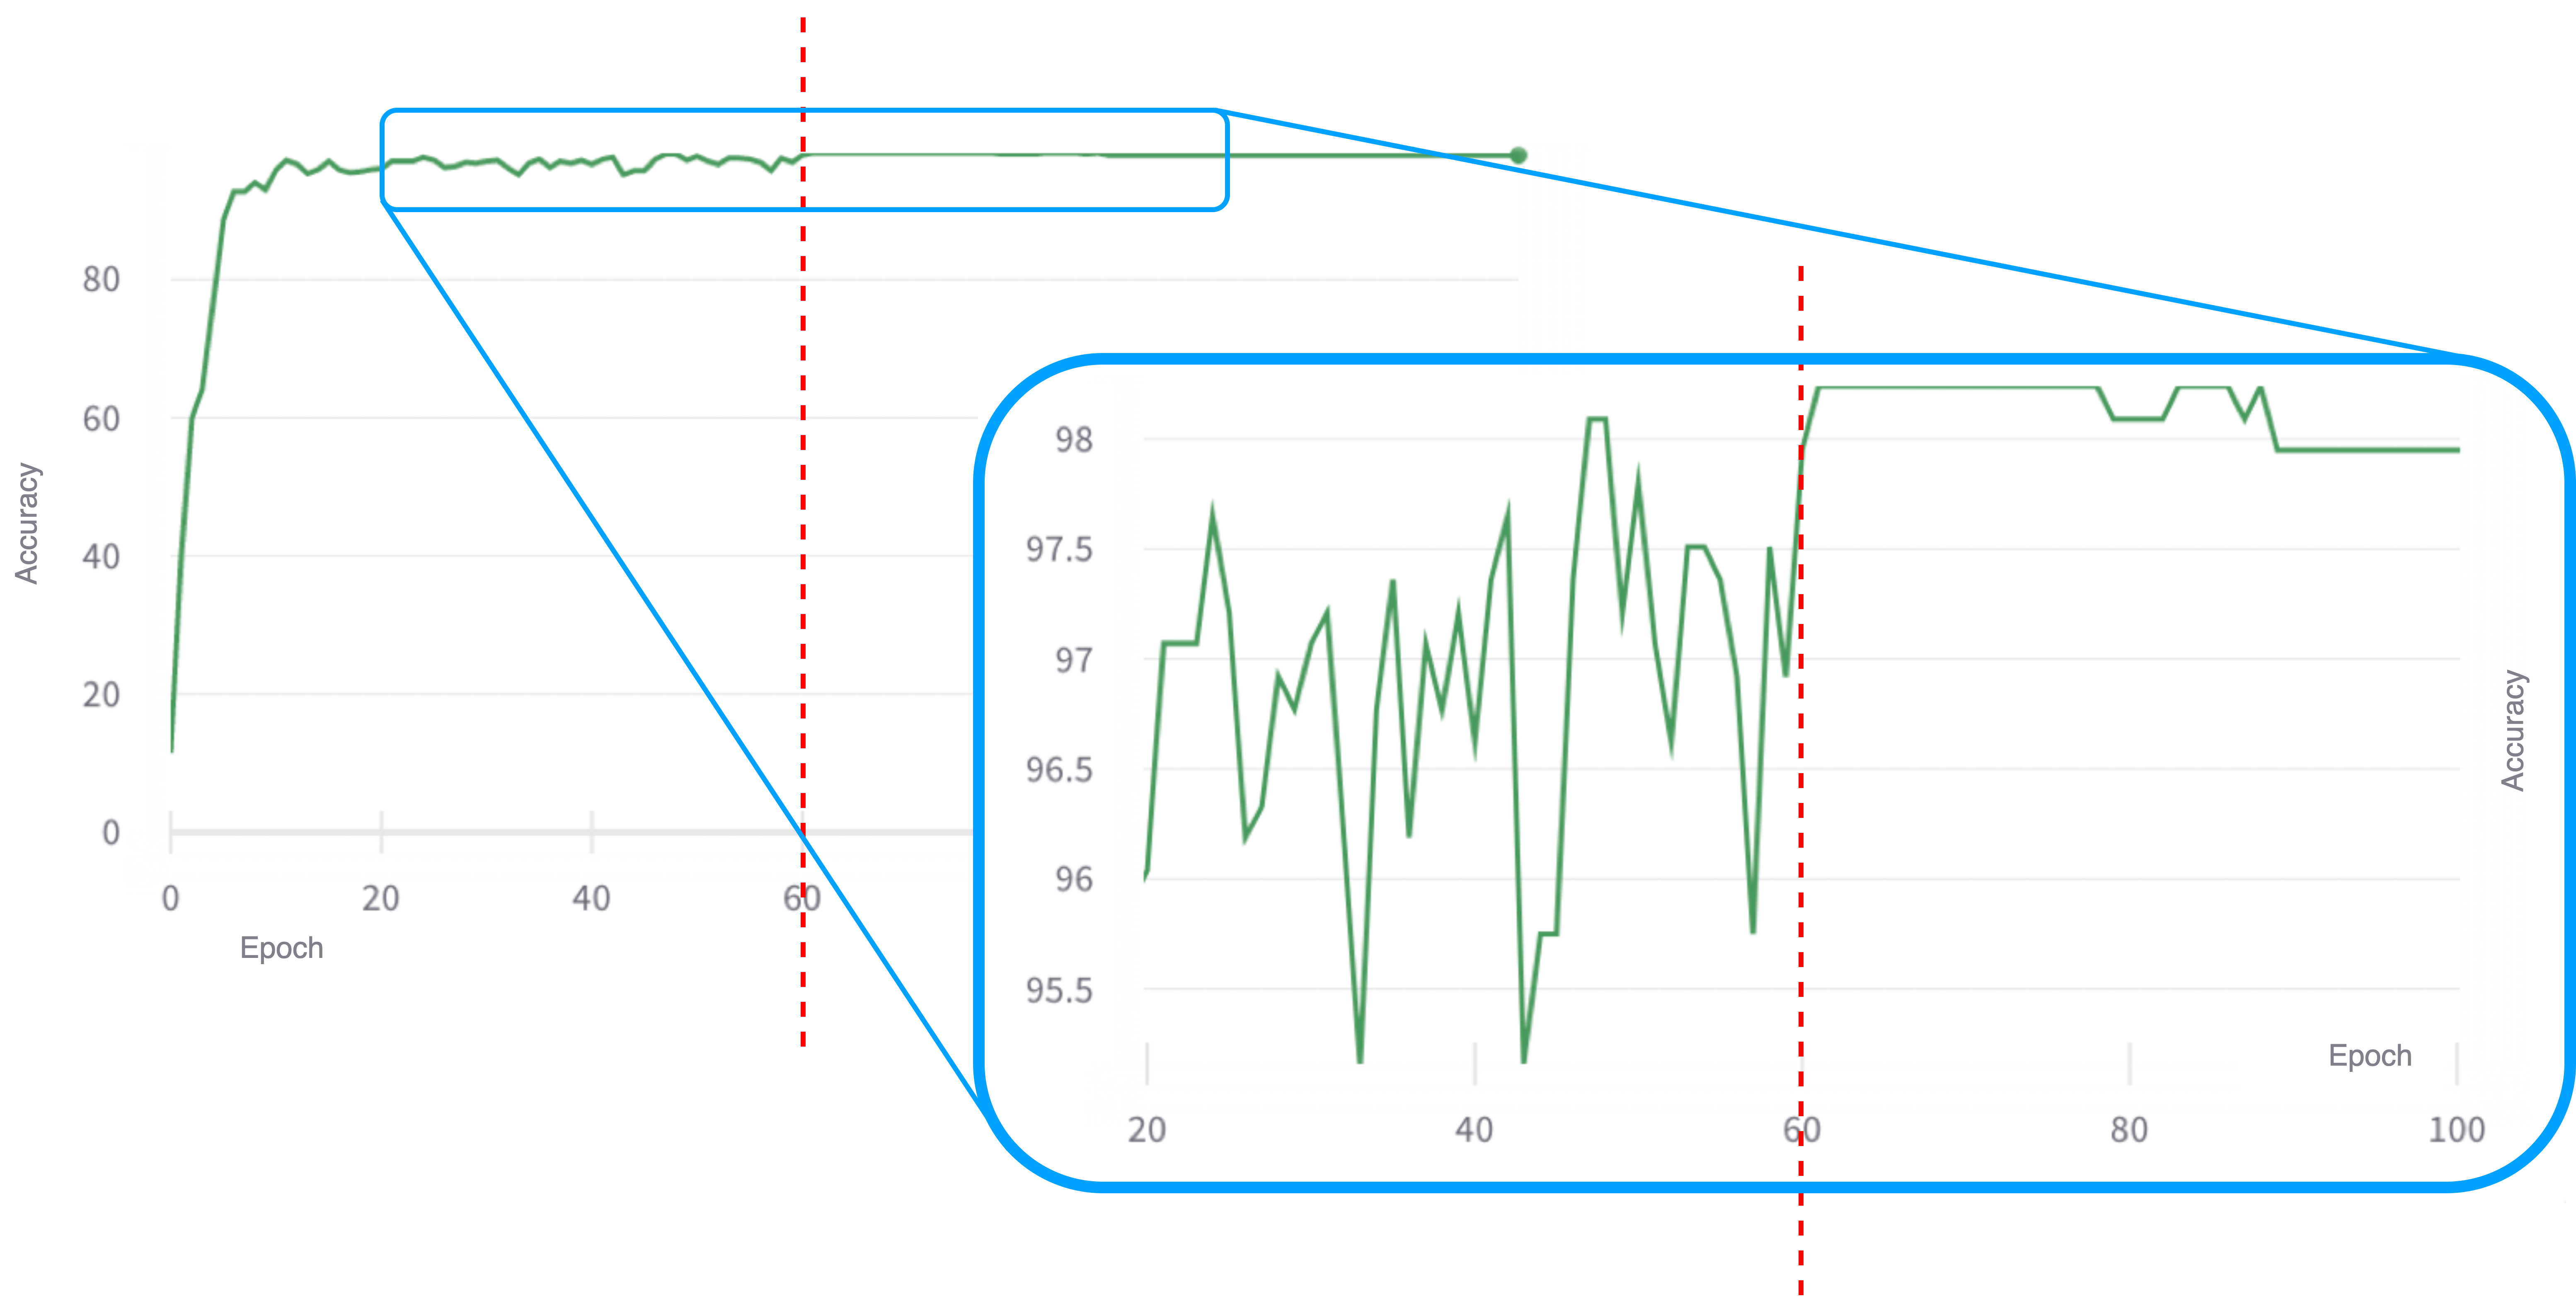
\includegraphics[width=\columnwidth]{images/lr_decay.drawio.png}
    \end{center}

	\caption{Effect of the learning rate decay: the figure shows the accuracy of the model at each training epoch. At epoch 60, the learning rate is scaled by a factor of $10^{-1}$, this leads to an increase in the model's accuracy in subsequent epochs.}
	\label{fig:lr_decay}%
\end{figure}


\subsection{Pruning}
\label{sec:method-pruning}

The DER algorithm, described in \autoref{sec:der-algorithm}, addresses the problem of class incremental learning by expanding the neural network architecture at each incremental step. The super-feature extractor at step $t$ of incremental learning is given by the following concatenation $\Phi_t(\mathbf{x}) = [\mathcal{F}_0, \, \mathcal{F}_1(\mathbf{x}), \, ..., \, \mathcal{F}_t(\mathbf{x})]$. As discussed in \autoref{sec:resnet}, the feature extractor is a CNN, which in this thesis is implemented using ResNet-34.

Given the definition of the super-feature extractor, it is possible to see how the parameters of the neural network grow linearly as a function of the number of incremental learning steps.
It is important to note that as the parameters of the super-feature extractor increase, those of the classifier $\mathcal{H}_t$ do as well.
The classifier $\mathcal{H}_t$ corresponds to the fully connected layer of the neural network. At each incremental learning task new classes are introduced, thus new connections are created between the classifier predicting the output class and the super-feature extractor.

This means that, using the LogoDet-3K dataset described in \autoref{chap:dataset}, and the incremental learning setup described in \autoref{sec:whole_dataset_clf}, at the 8th step of CIL the total number of parameters is given by: the number of parameters at task 0 (initial task), in which 22 million parameters (number of parameters of ResNet-34) are used; the 8 incremental learning steps, each adding 22 million parameters to the total.

After only 8 iterations of incremental learning, the final neural network reaches 205 million parameters, which is a large number of parameters compared to a single ResNet-34 used as backbone of each feature extractor.
For this reason, there is a need to reduce the number of parameters of the neural network.
To do so, the pruning of the network is implemented using masks, as described in \autoref{sec:masking-pruning}.

Each mask $\mathbf{m}_l$ associated with the channels of each layer $l$ of the CNN is computed as shown in \autoref{eq:mask}.
At the incremental learning task $t$, after the training of the feature extractor $\mathcal{F}_t(\mathbf{x})$, the variable $s$ is set to a really high value ($10^{4}$ in the implementation).
Since $s$ is fed into the sigmoid used as gating function, a steep activation mechanism is obtained (which leads to a binary activation when the limit of $s$ tends to infinity, but this behavior is achieved in practice using high value of $s$).
So, if a value $e_{li}$ of the mask $\mathbf{e}_l$ is positive, $m_{li}$ tends to 1, else if $e_{li}$ is negative, $m_{li}$ tends to 0.
To perform the actual binarization of each mask value, a threshold $\tau$ with a low value set to $10^{-4}$ is used as follows:

\begin{align*}
    m_{li}&=\left\{
        \begin{array}{@{}ll@{}}
            1, & \text{if } m_{li} > \tau\\
            0, & \text{if } m_{li} \leq \tau\\
        \end{array}\right.\\
\end{align*}

An important aspect to consider during the pruning of each convolutional layers $l$ of the feature extractor $\mathcal{F}_t(\mathbf{x})$ is the input and output dimension of the feature maps.
Since $\mathbf{m}_l$ is a channel-level mask, the effect of pruning is to reduce the number of channels in the convolutional layers of the CNN.
This results in a change in the output dimension of the convolutional layer $l$, so the input dimension of the convolution $l+1$ must be consistent with that output dimension.

Another point to consider is the architecture used to implement the feature extractors $\mathcal{F}_t$. In fact, each feature extractor has ResNet-34 as its backbone, which is an architecture based on residual connections (see \autoref{table:resnet} and \autoref{fig:residual-connection}).
This is a limitation from a pruning perspective: as mentioned above, each feature map produced as output from one convolutional layer must have a consistent dimension with the input next one;
in addition the residual connection adds a new constraint relative to the input dimension of convolutional layers. This issue is shown and described in \autoref{fig:pruning-resnet}.


\begin{figure}[H]
    \begin{center}
        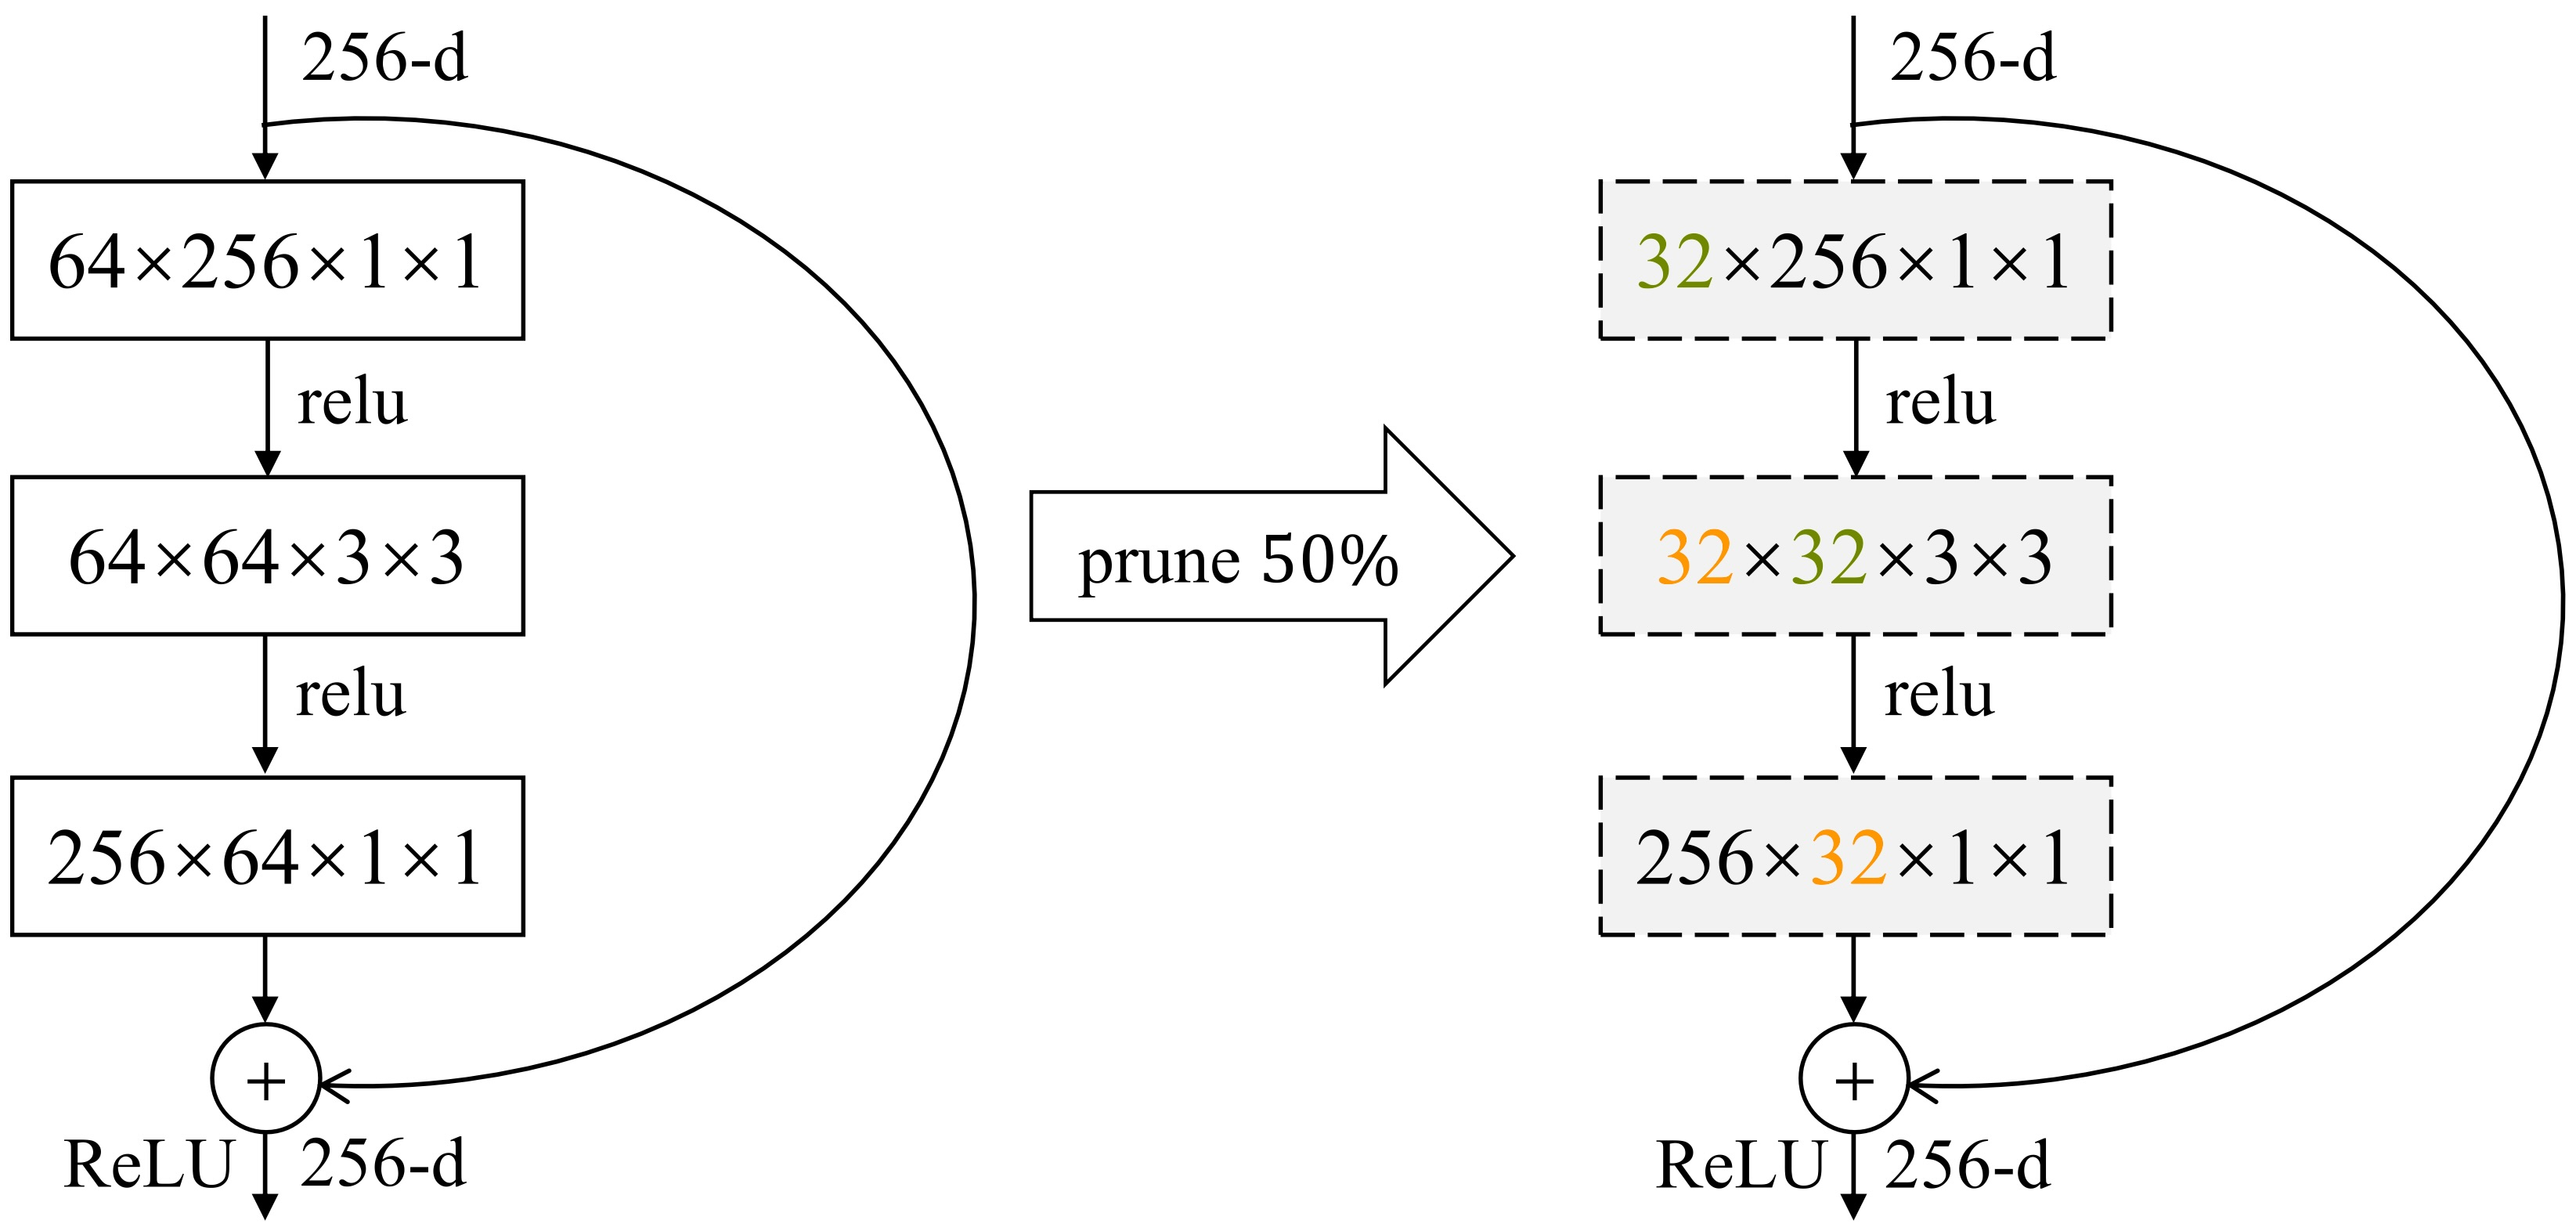
\includegraphics[width=\columnwidth]{images/resnet-pruning.png}
    \end{center}
    \caption{Pruning strategy of ResNet. The pruning is performed in such a way that the final size of the output is maintained, so that the residual connection can be added. Image from \cite{8416559}.}
    \label{fig:pruning-resnet}
\end{figure}

The use of residual connections involves pruning at the block level.
The definition of a block depends on the specific  architecture of ResNet. In the case of ResNet-34, a block consists of two convolutional layers, as shown in \autoref{table:resnet}, so pruning is applied to pairs of convolutions in order to add the identity carried by the residual connection.

\section{Knowledge distillation}
\label{sec:method-kd}

\begin{figure}[H]%
	\centering

    \begin{center}
        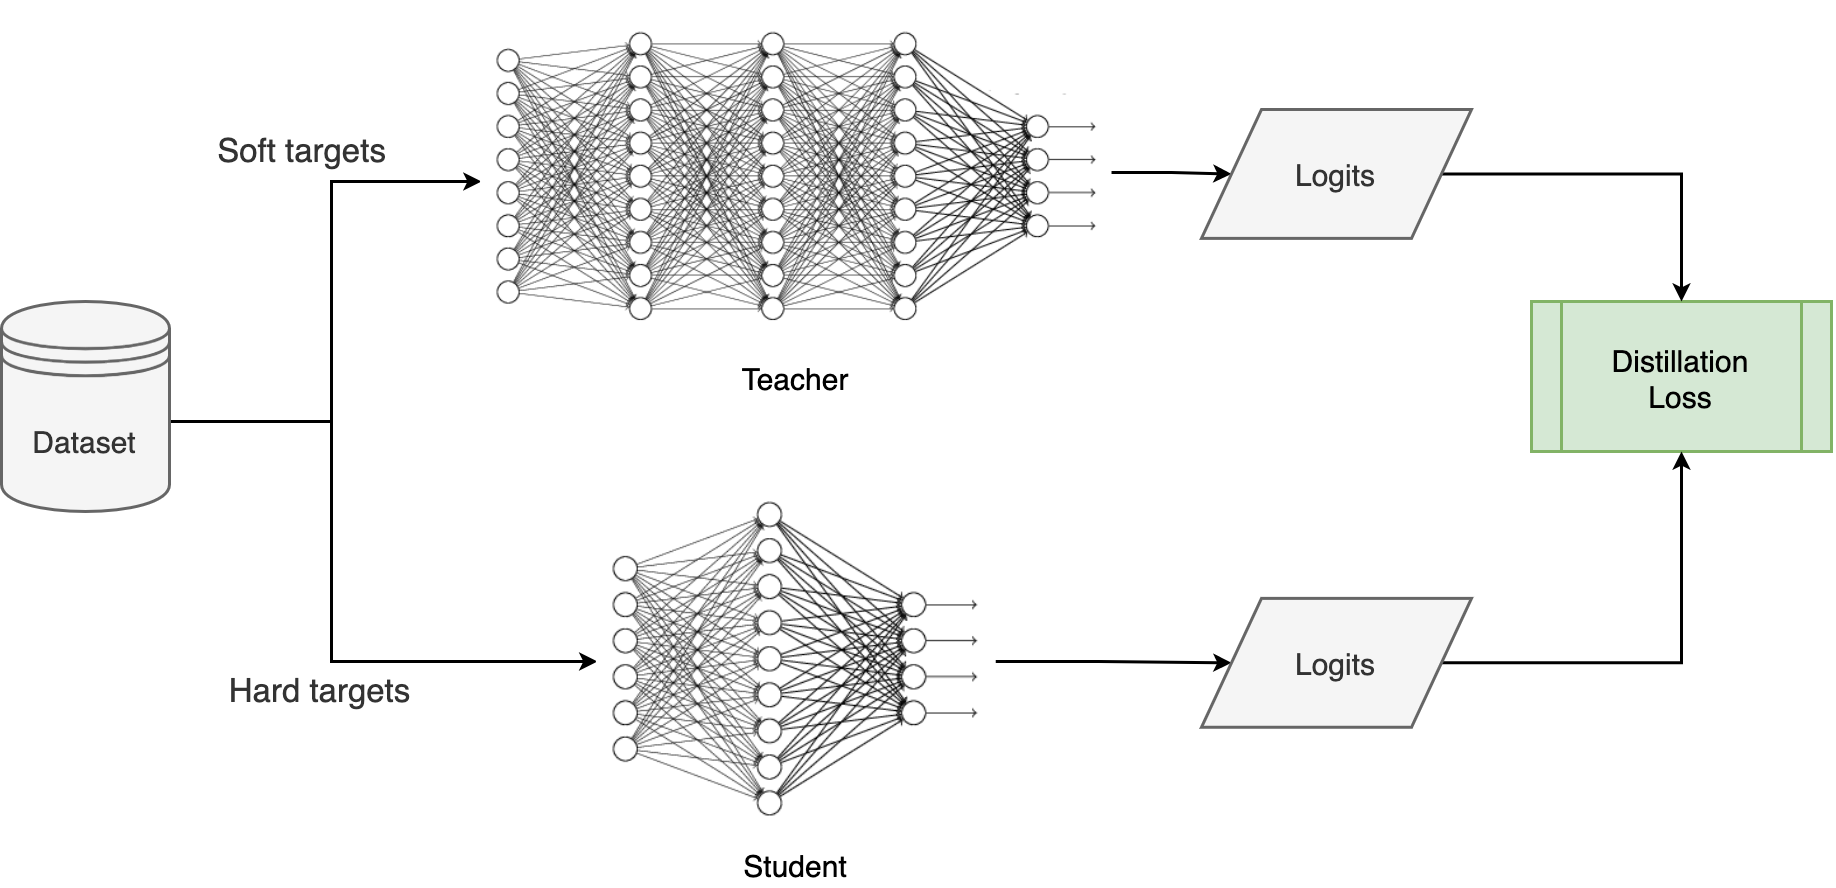
\includegraphics[width=\columnwidth]{images/kd.drawio.png}
    \end{center}

	\caption{Knowledge distillation pipeline: the student model is trained by exploiting the teacher model using the distillation loss. This loss considers both the logits of the teacher and the real data labels.}%
	\label{fig:kd}%
\end{figure}

Another approach used to tackle the problem of the large number of model parameters, described in the previous section, is Knowledge Distillation (KD) \cite{hinton2015distilling}. KD is the process of transferring knowledge from a pre-trained large model to a smaller one. Even if large models (such as very deep neural networks like ResNet-152) have higher knowledge capacity than small models, this capacity might not be fully exploited. A large model with regularization (e.g. dropout) generalizes better than a small model when trained directly on the data and labels, however, a small model can be trained to generalize better with the help of a large model. This training setting is referred to as 'teacher-student', where the smaller model is the student and it is trained to mimic the larger one which is the teacher.

As described by Gou et al. in \cite{gou2021knowledge},
Response-Based Knowledge is a type of KD which refers to the output layer of the teacher model.
In this thesis, the implementation of the KD is based on the paper of Hinton et al. in \cite{hinton2015distilling}.
The main idea is to directly mimic the final prediction
of the teacher model.
The reason behind this is that the output probabilities of a trained model give more information than the raw labels, because they assign non-zero probabilities to incorrect classes.
Knowledge is transferred from the teacher to the student using a loss function, known as the distillation loss, which captures the differences between the logits of the student and teacher models.
As the loss is reduced over time, the student becomes more accurate in making predictions similar to those of the teacher.
The teacher-student setting for KD matching the logits between the two models is shown in \autoref{fig:kd}.

The distillation loss used to train the student model is computed considering both the logits produced in output by the teacher (soft targets) and the real data labels (hard targets).
The probability $p_i$ of each class $i$, is computed by the teacher model using its logit $z_i$ as follows:
\begin{equation}
    p_i = \frac{exp(z_i)}{\sum_j exp(z_j)}
\end{equation}

The small model is trained to minimize the KL Divergence between its output probability distribution and the one of the large network.
One issue with this technique is that the probabilities assigned to incorrect classes by the large network are often very small and do not contribute to the loss.
For this reason, the logits are softened using a 'temperature' $T$ in the softmax, smoothing the probability distribution and revealing inter-class relationships learned by the teacher.
Then, the softened probability is given by:
\begin{equation}\label{eq:kd_prob}
    p_i^t = \frac{exp(\frac{z_i^t}{T})}{\sum_j exp(\frac{z_i^t}{T})}
\end{equation}
where higher values of $T$ produce softer probabilities. The prediction $p_i^t$ is called soft target, shown in \autoref{fig:kd}. 
Note that the teacher's output probability is denoted by $p_i^t$ using the letter $t$, as opposed to the student's output probability denoted by $p_i^s$ with the letter $s$.

Similarly, the \autoref{eq:kd_prob} is used to compute the class probability $p_i^s$ predicted by the student using its logit $z_i^s$ and the same temperature $T$.
In addition to the soft targets of the teacher, Hinton et al. in \cite{hinton2015distilling} show that it is also beneficial to train the student model to produce the real data labels, called hard targets and shown in \autoref{fig:kd}.
Therefore, by setting $T = 1$, the student uses \autoref{eq:kd_prob} to compute the 'standard' class probability $\hat{y}_i^s$.

Thus, considering both the KL divergence of the output probability distribution, and the Cross-Entropy between $\hat{y}_i^s$ and the true data label $y_i$, the final distillation loss is given by:
\begin{equation}
    \mathcal{L}_{KD} = \alpha \left[\sum_{i=1}^{\substack{\text{output}\\\text{size}}} p_i^t \, log \left( \frac{p_i^t}{p_i^s} \right) \right]
    + (1-\alpha) \left[-\sum_{i=1}^{\substack{\text{output}\\\text{size}}} y_i^s \, (\log \hat{y}_i^s) \right]
\end{equation}
where $\alpha \in [0, 1]$ is a hyper-parameter controlling the weighted average between the two components.

\section{Proposed baseline for the classifier}
\label{sec:method-baseline}
To evaluate the CIL models and compare their performance with a model in a traditional setup, it is necessary to define a baseline.
The CIL setup is very useful for introducing new classes after training, but in general this advantage is at the expense of the model's performance. Consequently, a CIL model performs worse than a traditional one, but a good CIL algorithm should narrow this gap in performance as much as possible.

Without considering the CIL aspect, different approaches can be defined to handle a classical classification problem. This chapter discusses the different baselines introduced with the aim of comparing them with the CIL models.

\subsection{Baseline without incremental steps}
\label{sec:method-baseline1}
The most direct approach is to define a baseline using the DER algorithm.
This means taking all the classes introduced at each iteration of incremental learning and using them from the very beginning, at task 0, to train the model with the DER algorithm.
The process described above defines the first type of baseline.

Although this approach appears to be simple and straightforward, it has a problem related to what is described in \autoref{sec:method-pruning}. In fact, such an approach is not very fair, as the baseline has a number of parameters $N$ equal to the CNN used as the backbone for the feature extractor, while the CIL model trained with the DER algorithm has a number of parameters equal to $N + t \times N$ (where $t$ is the number of iterations of incremental learning).
As a result, the CIL model may perform better than the baseline only because it has a significantly larger number of parameters.

\subsection{ResNet-152 architecture}
\label{sec:method-baseline2}
In order to solve the problem of the first baseline definition, relating to the difference in parameters between the baseline and the CIL model, a second type of baseline is defined.
In this second approach, the DER algorithm is no more exploited, instead it is used ResNet-152 which is a network with a significantly higher number of parameters compared to ResNet-34. This is done to bridge the gap of the number of parameters between the baseline and the CIL model. The CNN based on ResNet-152 is then trained for the classification task considering all the classes.

The architecture of ResNet-152 is very similar to the one described in table \autoref{table:resnet}, in fact it maintains all the main features such as skip-connections, but has each block composed of more convolutional layers, and the number of stacked blocks increases. The architecture of ResNet-152 consists of 60 million parameters and is described in \autoref{table:resnet-152}.


\begin{table}
    \centering
    \begingroup
    
    \begin{tabular}{>{\centering\arraybackslash}p{.3\textwidth}|>{\centering\arraybackslash}p{.3\textwidth}|>{\centering\arraybackslash}p{.3\textwidth}}


        \hline
        \multicolumn{3}{c}{\textbf{ResNet-152 architecture}}\\
        \hline
        \textbf{Layer name} & \textbf{Output size} & \textbf{Layer} \\
        \hline
        \hline
        conv1 & $112 \times 122$ & $7 \times 7, 64,$ stride $2$ \\
        \hline
          & $56 \times 56$ & $3 \times 3$ max pool, stride $2$ \\
        \hline

        \[ \textrm{conv2\char`_x} \] &  \[56 \times 56 \] & \[\left[ \begin{array}{c} 1 \times 1, \, 64\\ 3 \times 3, \, 64 \\ 1 \times 1, \, 256  \end{array} \right] \times 3 \]\\
        \hline

        \[ \textrm{conv3\char`_x} \] &  \[28 \times 28 \] & \[\left[ \begin{array}{c} 1 \times 1, \, 128 \\ 3 \times 3, \, 128  \\ 1 \times 1, \, 256  \end{array}\right] \times 8 \]\\
        \hline

        \[ \textrm{conv4\char`_x} \] &  \[14 \times 14 \] & \[\left[ \begin{array}{c} 1 \times 1, \, 256\\ 3 \times 3, \, 256\\ 1 \times 1, \, 1024  \end{array}\right] \times 36 \]\\
        \hline

        \[ \textrm{conv5\char`_x} \] &  \[7 \times 7 \] & \[\left[ \begin{array}{c} 1 \times 1, \, 512\\ 3 \times 3, \, 512\\ 1 \times 1, \, 2048  \end{array}\right] \times 3 \]\\
        \hline
        & $1000 \times 1$ & average pool \\
        \hline
        FC & $1000 \times 1$ & $1000$-d FC layer, softmax \\
        \hline
        \end{tabular}
    \endgroup
    \caption{Architecture of ResNet-152, the brackets represent a stack of building blocks.}
    \label{table:resnet-152}
\end{table}

Although this new baseline is an improvement over the previous one, the number of parameters may still be lower than in the CIL model, as in the case of the baseline of the first type.

\subsection{DER-based architecture}
\label{sec:method-baseline3}
The third introduced baseline solves the problem of the different number of parameters between the CIL model and the baseline.
To this purpose, referring to the exact same setup used for training the CIL model and considering the number of iterations $t$, the DER algorithm is exploited to define another neural network by performing $t$ incremental learning steps without actually training the new network.
Subsequently, since at timestamp $t$ of incremental learning the DER algorithm freezes the weights of the feature extractors associated with the timestamps $t-1$, all weights, both relative to the feature extractors $\mathcal{F}_i$ and to the classifier $\mathcal{H}_{i}$, are allowed to be trained.

This new network will serve as the baseline, and unlike the DER algorithm, the optimization process will aim to classify all the classes (intended as all those introduced incrementally during the training of the CIL model) without taking into account the auxiliary classifier $\mathcal{H}^a$ and the masks for pruning described in \autoref{sec:der-algorithm}.